\chapter{DNS Rebinding}

To reiterate, DNS rebinding is a computer attack, for which an attacker subverts
the same-origin policy of browsers, by running a client-side script used to
attack target machines on a network, and converts them into open network
proxies\textsuperscript{\cite{jackson2009protecting}}.

\vspace{0.5cm}

\begin{figure}[H]
\begin{center}
	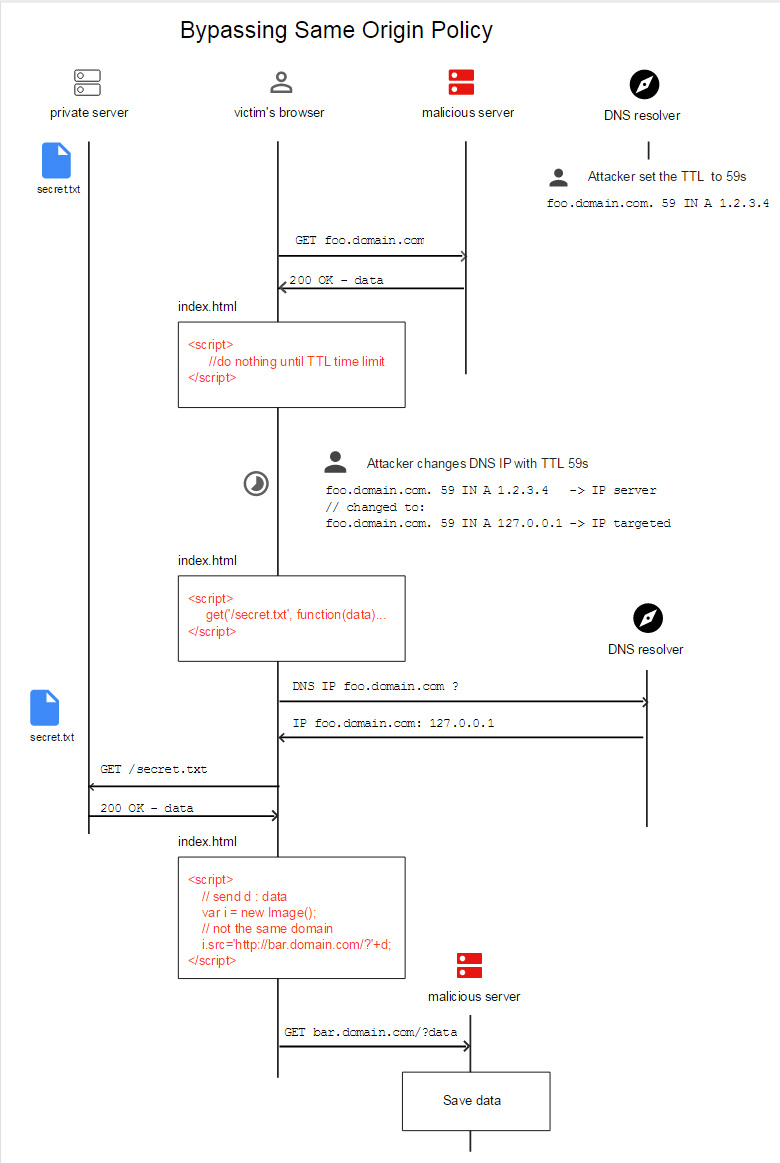
\includegraphics[width=0.59\textwidth,keepaspectratio]{img/dnsrebindingflow.jpg}
	\caption{DNS Rebinding Flow Diagram\textsuperscript{\cite{vulnsec}}}
\end{center}
\end{figure}

\vspace{0.5cm}

An attacker would register a domain and assign it to a DNS server under their
control. When a target/victim visits the attacker's domain, the DNS server
initially responds with the IP address of a server which contains malicious
client-side scripts (JavaScript or Flash). The code makes additional accesses
to the original domain, which is permitted by the SOP. However when the
target's browser runs the script, a new DNS request is made for the original
domain and the attacker replies with a new IP address.

\section{Types of DNS Rebinding}

\subsection{Multiple A Records}

\subsection{Time-Varying DNS}
